\section{Vlastnosti kombinačních čísel}

V této sekci se budeme \emph{především} (avšak ne vždy) držet naší původní definice kombinačního čísla z \ref{def:kombinacni_cislo}, tj.
\[\binom{n}{k}=\dfrac{n(n-1)(n-2)\cdots(n-k+1)}{k!},\]
a to právě kvůli již zmíněné vlastnosti, že oproti
\[\dfrac{n!}{(n-k)!k!}\]
dává výraz smysl i pro $k>n$ a je vždy roven nule (ostatně i z kombinatorického hlediska dává tento výsledek smysl). Nebudeme se tak muset explicitně odvolávat na předpoklad, že $n\leqslant k$, abychom předešli formálním nepřesnostem.
\medskip

U kombinačních čísel lze pozorovat některé zajímavé vlastnosti. Začneme asi tou nejzákladnější.
\begin{theorem}[Symetrie kombinačních čísel]\label{thm:symetrie_kombinacnich_cisel}
    Pro $n,\,k\in\N_0$, kde $k\leqslant n$, platí
    \[\binom{n}{k}=\binom{n}{n-k}.\]
\end{theorem}
\begin{proof}[Důkaz první]
    Asi nejjednodušší důkaz je přímým výpočtem:
    \[\binom{n}{n-k}=\dfrac{n!}{(n-(n-k))!(n-k)!}=\dfrac{n!}{k!(n-k)!}=\binom{n}{k}.\]
\end{proof}
\begin{proof}[Důkaz druhý]
    Názornější důkaz nám poskytne kombinatorická interpretace tohoto tvrzení. Libovolná $k$-tice (v tomto smyslu množina) je \textbf{jednoznačně určena} výběrem prvků z nějaké $n$ prvkové množiny, které jí budou náležet. Výběrem $k$ prvků z dané množiny tak zbude $n-k$ prvků, které nejsou součástí dané $k$-tice.
    \begin{figure}[H]
        \centering
        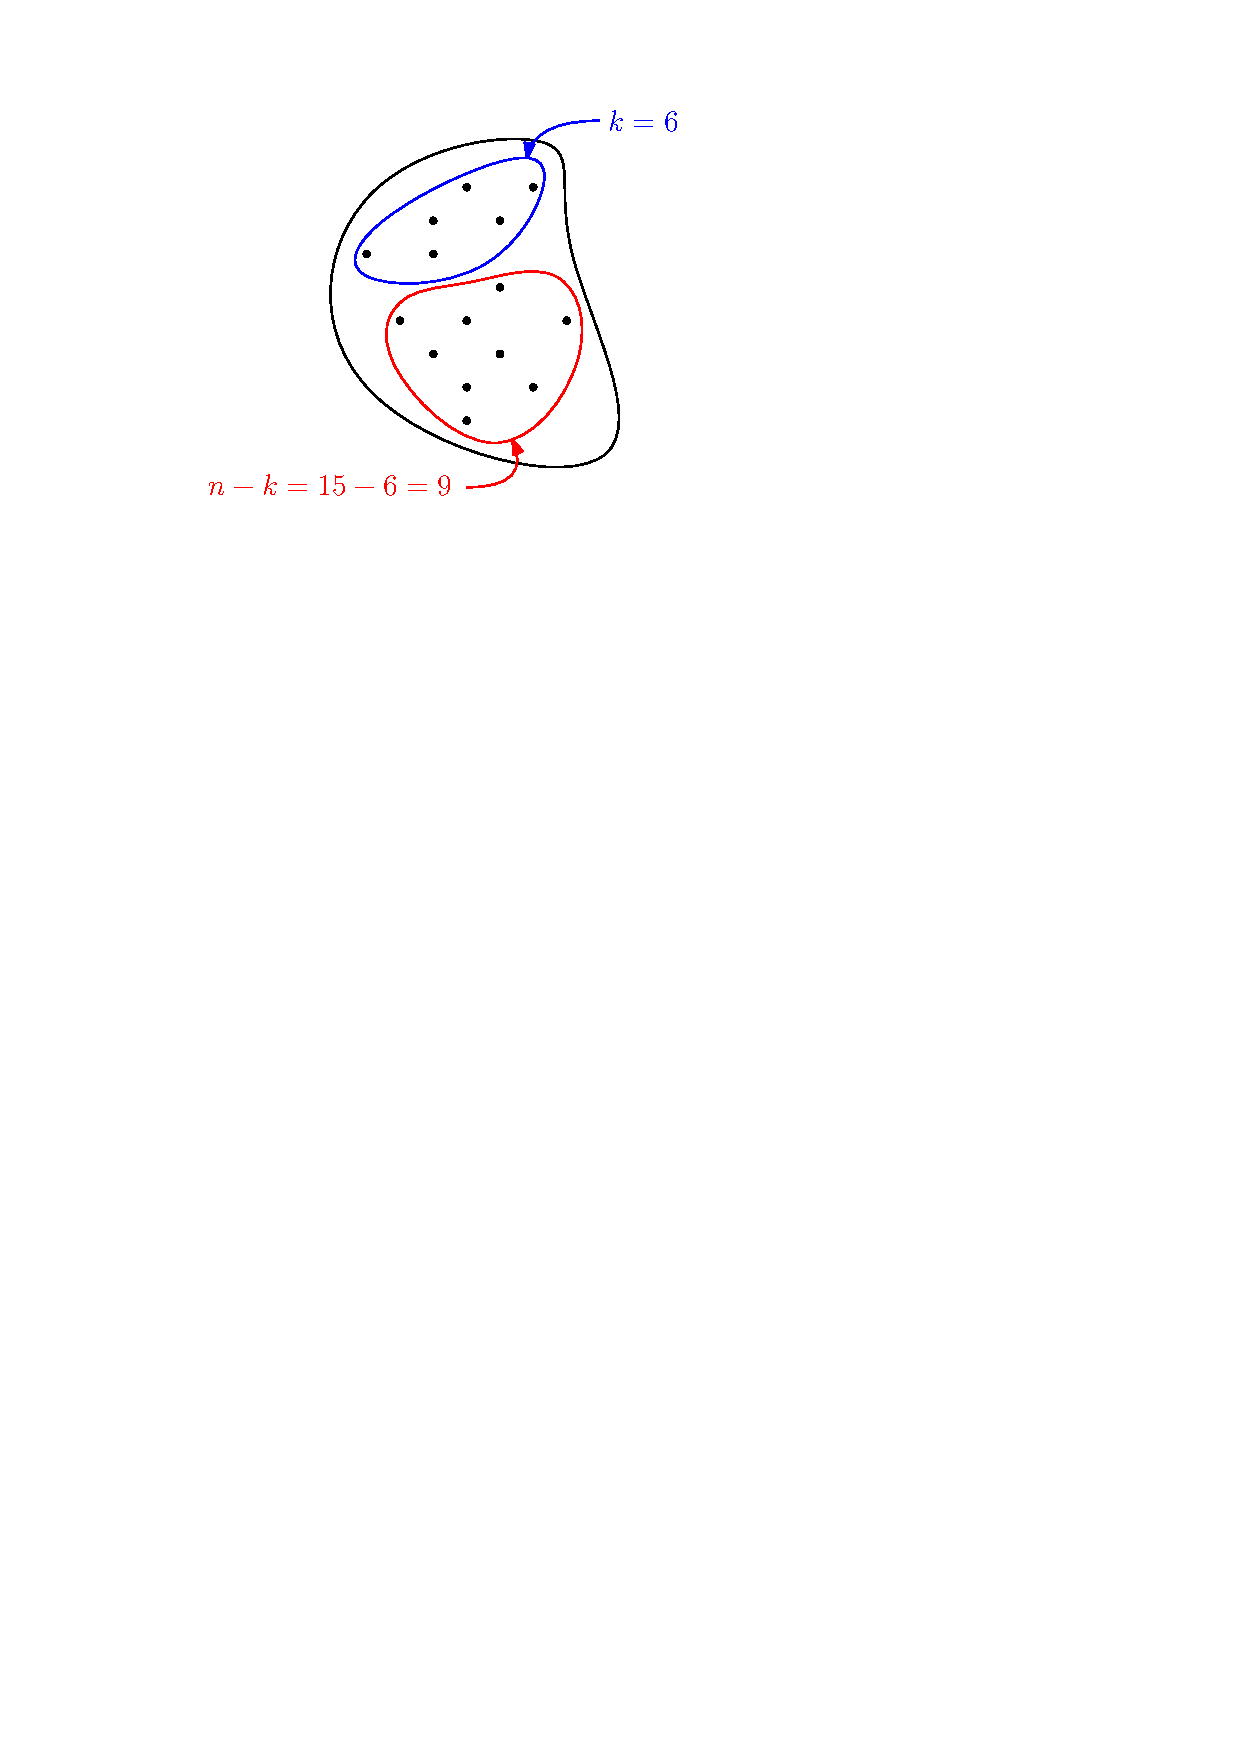
\includegraphics[scale=\normalipe]{ch03_podmnoziny.pdf}
        \caption{Výběr šesti prvků z patnácti.}
        \label{fig:podmnoziny}
    \end{figure}
    Takových možných výběrů existuje $\binom{n}{k}$. Danou $k$-tici ovšem lze vybrat i opačným způsobem, a to sice volbou prvků, které jí náležet \textbf{nebudou}. Tedy výběrem $n-k$ prvků zbude celkem $k$ prvků, které jí budou náležet. Takových výběrů existuje $\binom{n}{n-k}$. Protože výběrem $n-k$ prvků vždy jednoznačně určíme nějakou $k$-tici, pak neuspořádaných $k$-tic a neuspořádaných $(n-k)$-tic musí být stejně, tj.
    \[\binom{n}{k}=\binom{n}{n-k}.\]
\end{proof}

\begin{theorem}\label{thm:soucet_kombinacnich_cisel}
    Pro $n,\,k\in\N_0$ platí
    \[\binom{n}{k}+\binom{n}{k+1}=\binom{n+1}{k+1}.\]
\end{theorem}
\begin{proof}[Důkaz první]
    Obdobně i zde lze tvrzení dokázat přímým výpočtem:
    \begin{align*}
        \binom{n}{k}+\binom{n}{k+1}&=\dfrac{n(n-1)\cdots(n-k+1)}{k!}+\dfrac{n(n-1)\cdots(n-k+1)(n-k)}{(k+1)!}\\ &=\dfrac{n(n-1)\cdots(n-k+1)}{k!}\cdot\left(1+\dfrac{n-k}{k+1}\right)\\ &=\dfrac{n(n-1)\cdots(n-k+1)}{k!}\cdot\dfrac{n+1}{k+1}\\ &=\dfrac{(n+1)n(n-1)\cdots(n-k+1)}{(k+1)!}=\binom{n+1}{k+1}.
    \end{align*}
\end{proof}
\begin{proof}[Důkaz druhý]
    Opět o něco názorněji lze platnost tvrzení zdůvodnit kombinatorickou úvahou. Představme si, že máme množinu
    \[\set{1,\,2,\,\dots,\,n,\,n+1}.\]
    Chceme vybrat spočítat počet možných výběrů všech neuspořádaných $(k+1)$-tic, pak jejich počet odpovídá kombinačnímu číslu $\binom{n+1}{k+1}$. To je význam pravé strany rovnosti.\par
    Chceme-li vybrat všechny neuspořádané $(k+1)$-tice, lze postupovat i následovně:
    \begin{itemize}
        \item vybereme všechny $(k+1)-tice$, které \textbf{obsahují prvek $n+1$} a
        \item vybereme všechny $(k+1)$-tice, které \textbf{neobsahují prvek $n+1$}.
    \end{itemize}
    Je nejspíše intuitivně jasné, že neuspořádané $(k+1)$-tice z obou skupin dají celkově všechny $(k+1)$-tice (každá z nich buď daný prvek obsahuje, nebo jej neobsahuje). V prvním případě máme jeden prvek již vybraný, a to $n+1$. Zbylých $k$ prvků lze vybrat $\binom{n}{k}$ způsoby.\par
    V druhém případě vybíráme $k+1$ prvků, avšak pouze z $n$ prvků (prvek $n+1$ neuvažujeme). Takových výběrů existuje $\binom{n}{k+1}$. Protože obě "skupiny" neuspořádaných $(k+1)$-tic jsou disjunktní, je tak celkový všech $k+1$-tic z $n+1$ prvků roven
    \[\binom{n}{k}+\binom{n}{k+1}.\]
\end{proof}